\section{Clase 13}
\subsection{Fermiones a baja temperatura}
Tenemos
	\begin{equation}
  f(\ep-\m,T )=\frac{e^{-(\ep-\m )/\k T}}{1+e^{-(\ep_\m )/\k T}}
\end{equation}
para $\k T\ll\m $ uno puede expandir $f$ en la vecindad de $\m$,
\begin{equation}
  f\approx f_0+\d f,\qquad f_0=\Th (\ep-\m )
\end{equation}
\begin{align}
  \d f&=\left\{\begin{array}{ll}
  	\dfrac{-e^{-\ep'/\k T}}{(1+-e^{-\ep'/\k T})}-1,& \quad \ep'=\ep-\m <0\\ \\
  	\dfrac{e^{-\ep'/\k T}}{(1+-e^{-\ep'/\k T})},&\quad \ep'>0
  \end{array}\right.
\end{align}
Podemos graficar $f(\ep)$,
\begin{figure}[h!]
	\centering
	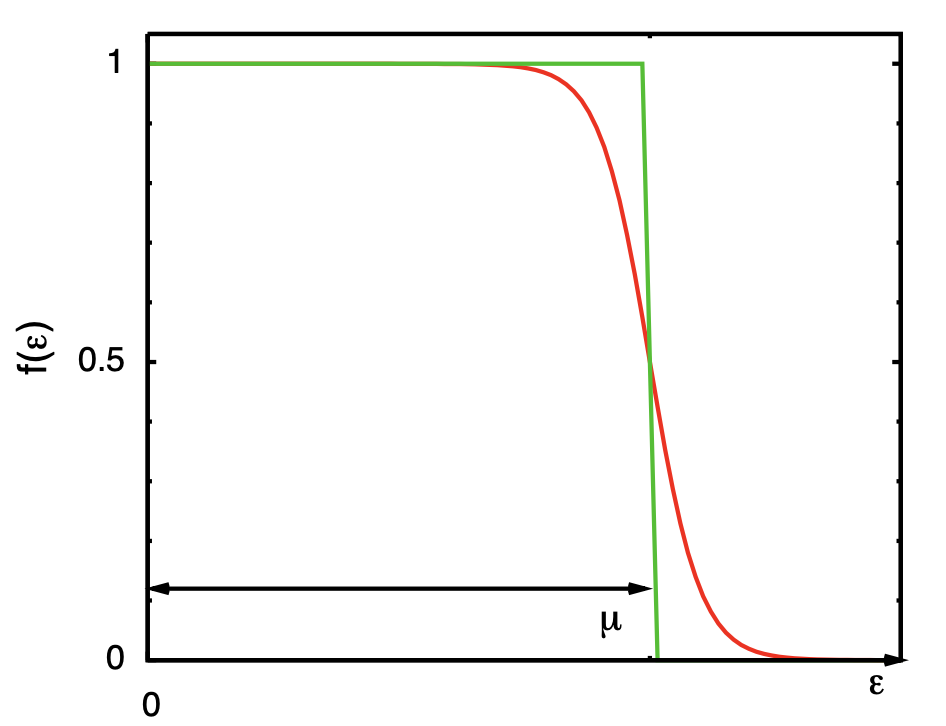
\includegraphics[scale=0.5]{fig/im1.png}
\end{figure}
y también $\d f(\ep')=f(\ep')-f_0(\ep')$ la cual es una función impar en $\ep'$, es decir, $\d f(\ep')=-\d f(-\ep')$,
Podemos graficar $f(\ep)$,
\begin{figure}[h!]
	\centering
	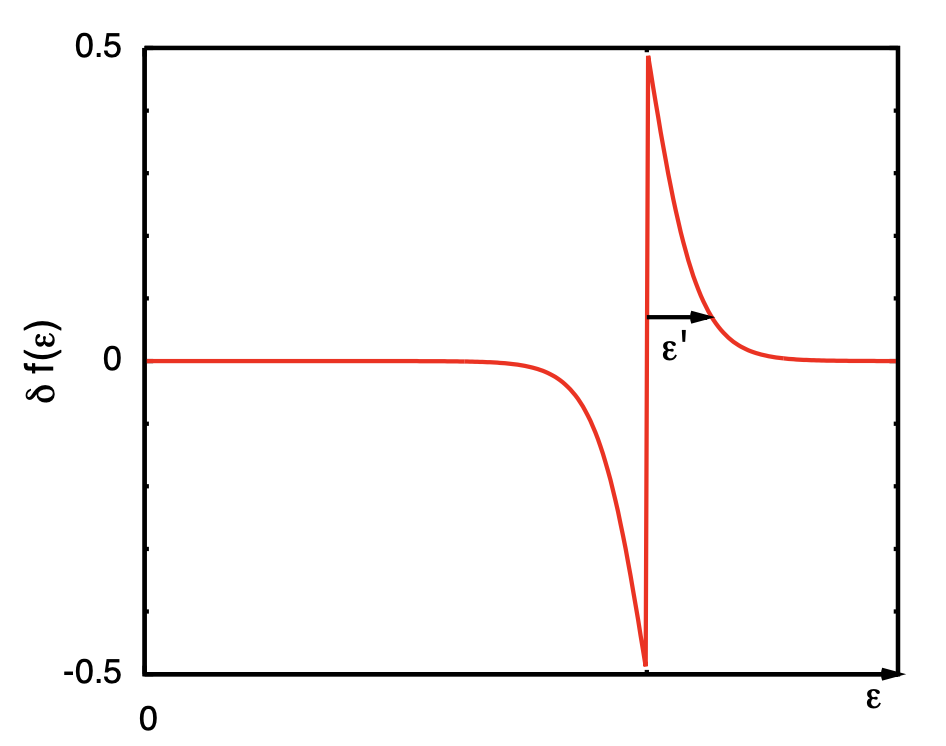
\includegraphics[scale=0.5]{fig/im2.png}
\end{figure}

También definimos la \textit{densidad de estados} como
\begin{equation}
  \frac{D(\epsilon)}{V}=\frac{1}{V}\dv{N}{p}\dv{p}{\ep}
\end{equation}
donde $D(\epsilon)$ corresponde al número de estados disponibles con energía entre $\ep$ y $\ep+\dd \ep$. Esta cantidad en $3$-dimensiones viene dada por
\begin{equation}
 \boxed{ \frac{D(\epsilon)}{V}=\frac{(2s+1)}{(2\p\hbar)^3}(4\p p^2)\dv{p}{\ep }}
\end{equation}

Expandiendo $D(\m+\ep')$ en potencias de $\ep'$, y para temperaturas pequeñas truncamos a primer orden,
\begin{equation}\label{13.star}
  \boxed{\frac{N}{V}=\r(\m,T)\approx \r(\m,T=0)+\frac{1}{V}\int_{-\infty}^\infty \dd\ep'\left[D(\m )+\ep'\eval{\dv{D(\ep)}{\epsilon}}_{\ep=\m }\right]\d f(\ep ')}
\end{equation}
Esto viene de considerar que
\begin{equation}
  \frac{N}{V}\r=\frac{1}{V}\int D(\ep )f(\ep-\m,T)\dd\epsilon
\end{equation}
y luego separar
\begin{equation}
  f(\ep-\m,T)=\underbrace{f_0(\ep-\m )}_{\Th (\m-\epsilon)}+\d f(\ep-\m,T)
\end{equation}
entonces
\begin{equation}
  \r=\underbrace{\frac{1}{V}\int_0^\infty D(\ep )\Th(\m-\epsilon)\dd\epsilon}_{\r(\m,T=0)}+\frac{1}{V}\int_0^\infty\dd\ep D(\ep )\d f(\ep-\m )
\end{equation}
Pero considerando $\ep'=\ep-\m$ y $\k T\ll \m $, puede aproximarse el rango de integración para $\ep'$ entre $-\infty$ y $\infty$. Entonces,
\begin{equation}
  \r=\r(\m,T=0)+\frac{1}{V}\int_{-\infty}^\infty \dd\ep' D(\ep'+\m )\d f(\ep ')
\end{equation}
Finalmente, usando serie de Taylor para $$D(\m+\ep')=D(\m )+\eval{\dv{D}{\ep }}_\m \ep'+\cdots $$ se obtiene \eqref{13.star}.

Para $\ev{E}/V\equiv E/V$ tenemos
\begin{equation}\label{13.star}
  \boxed{\frac{E}{V}= \frac{E}{V}(\m,T=0)+\frac{1}{V}\int_{-\infty}^\infty \dd\ep'(\m+\ep')\left[D(\m )+\ep'\eval{\dv{D(\ep)}{\epsilon}}_{\ep=\m }\right]\d f(\ep ')}
\end{equation}
Ahora para evaluar las integrales consideramos que $\d f(\ep')$ es una función impar en $\ep'$. Luego, tenemos
\begin{equation}
  \d\r \equiv \r(\m,T)-\r(\m,T=0)=\frac{2}{V}\eval{\dv{D	}{\epsilon}}_\m I(T)
\end{equation}
y
\begin{equation}
 \boxed{ \d\left(\frac{E}{V}\right)\equiv\frac{E}{V}(\m,T)-\frac{E}{V}(\m,T=0)=\m\d\r +\frac{2}{V}D(\m )I(T)}
\end{equation}
donde
\begin{equation}
  \boxed{I(T)\equiv \int_0^\infty \dd\ep'\ep'\frac{e^{-\ep'/\k T}}{1+e^{-\ep'/\k T}}=\k^2T^2\int_0^\infty \d x\frac{e^{-x}}{1+e^{-x}}}
\end{equation}

Verificamos $\d\r$,
\begin{equation}
  \d\r=\frac{1}{V}\int_{-\infty}^\infty\dd\ep'\left[D(\m )+\eval{\ep'\dv{D(\ep )}{\epsilon}}_\m \right]\d f(\ep')
\end{equation}
pero como $\d f$ es una función impar, $D(\m)\d f(\ep')$ también es impar. Luego,
\begin{equation}
  \int_{-\infty}^\infty\dd\ep'D(\m )\d f(\ep')=0
\end{equation}
\begin{equation}
  \implies \d\r=\frac{1}{V}\int_{-\infty}^\infty\dd\ep'\ep'\left[\eval{\dv{D(\ep )}{\epsilon}}_\m \right]\d f(\ep')
\end{equation}
pero el integrando es par. Si lo consideramos como un intervalo simétrico, se tiene
\begin{equation}
  \d\r=\frac{2}{V}\int_0^\infty\dd\ep'\ep'\left[\eval{\dv{D(\ep )}{\epsilon}}_\m \right]\d f(\ep ')=\frac{2}{V}\eval{\dv{D(\ep )}{\epsilon}}_\m I(T) 
\end{equation}
quedando así verificado.

Ahora verificamos $\d (E/V)$:
\begin{align}
  \d\left(\frac{E}{V}\right)&=\frac{1}{V}\int_{-\infty}^\infty\dd\ep'(\m+\ep')\left[D(\m )+\ep'\eval{\dv{D(\ep)}{\epsilon}}_{\ep=\m }\right]\d f(\ep ')\\
  &=\frac{1}{V}\int_{-\infty}^\infty\dd\ep'\left(\m D(\m )+\m \ep'\eval{\dv{D	}{\ep }}_{\m }+\ep' D(\m )+\ep'^2\eval{\dv{D}{\ep}}_\m \right)\d f(\ep' )
\end{align}
pero el primer termino se anula ya que el intervalos es par y $\d f$ es impar por lo que si se multiplica por una constante seguirá siendo impar. El último término igual se anula ya que $\ep'^2$ es par pero $\d f$ es impar, luego su producto es impar. \footnote{Recordemos que la integral de una función impar en un intervalo par es cero.}
















